\chapter{Motivation} \label{Chapter:motivation}

What I am actually looking at -  Compositionality, Problems of RNN- SCAN, Lookup Tables. Why should it be compositional.

Pondering should be here as well.


\section{Systematic Compositionality} \label{systematic}
Natural language and human reasoning arguably exhibit compositionality. Compositionality is the principle of understanding a complex expression through the meaning and syntactic combination of its morphemes. One of the strongest arguments in favor of compositionality is the presence of systematicty in natural language.

\textbf{Systematicity}. Provided [E1, E3] of same grammatical category and [E2,E4] of same grammatical category. If [E1,E2] can combine syntactically then so can [E1, E4], [E3, E2] and [E3,E4] and if one can understand ([E1,E2]) and ([E3, E4]) then they can also understand ([E1,E4]) and ([E3,E2]) provided that the is well formed.

The definition of compositionality presented above does not directly imply dependence on context in which the expression appears or the intent of the speaker and therefore the compositional nature of natural language is an active area of debate among linguists and philosophers \citep{sep-compositionality}. Aritifical languages (such as the ones we'll encounter in chapter \ref{Chapter:datasets}) on the other hand can be constructed to strictly follow the principles of systematic compositionality. Given human propensity for compositional solutions \citep{NIPS2016_6130} these datasets provide excellent test-beds for validating the existence of compositional skills in neural networks. 

\subsection{Compositionality in Seq2Seq Models}
Lake and Baroni concluded that seq2seq is still doesn't exhibit systematicity.

\subparagraph{Zero, One and Few shot generalization}

\section{Attention}

\subsection{Attention in Humans}
Attention from a cognitive neuroscience perspective. Attentional blink

\subsection{Se2Seq with Attention}
It was shown by \cite{Cho2014} that the performance of a basic encoder-decoder models as explained in \ref{background:s2s} is inversely related to the increase in length of the input sentence. Therefore in lines with concepts of the selective attention and attentional blink in human beings, \cite{Bahdanau2014} and later  \cite{Luong2015} showed that soft selection from source states where most relevant information can be assumed to be concentrated during a particular translation step in NMT leads to improved performance.

How is attention calculated? Equations? Plots? Also cover this from a key-value pair pov.

\section{Pondering}

\begin{figure}
	\begin{minipage}[t]{\textwidth}
		\ifpdf
		\includegraphics[width=\linewidth,keepaspectratio=true]{./figs/act-pdf}
		\else
		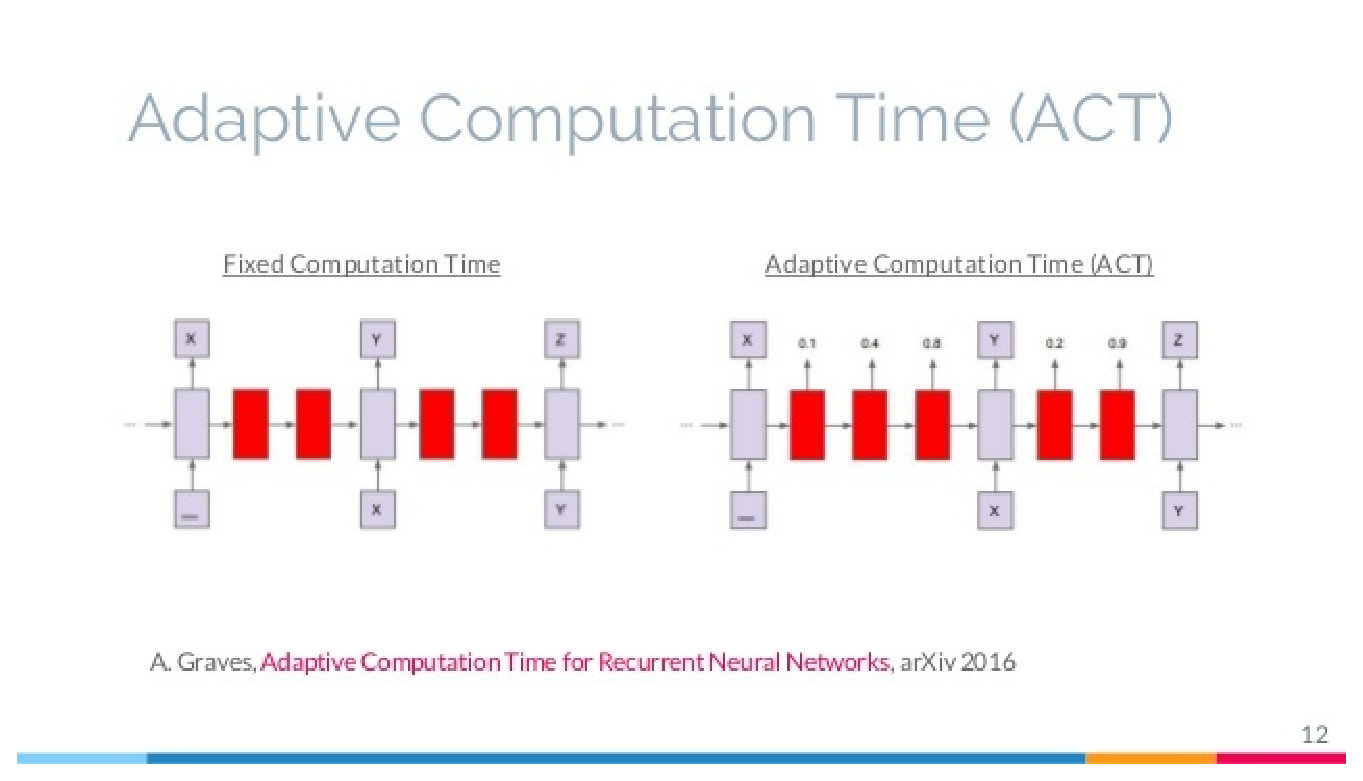
\includegraphics[width=\linewidth,keepaspectratio=true]{./figs/act-eps}
		\fi
		\caption{\small Adaptive Computation Time}
		\label{mtv:ponder}
	\end{minipage}
\end{figure}

The task of positioning a problem and solving belong to different classes of time complexity with the latter requiring more time than the former. \cite{Graves2016} argued that for a given RNN unit it is reasonable to allow for variable computation time for each input in a sequence since some parts of the input might be inherently more complex than the others and thereby require more computational steps. A very good example of this would be \textit{spaces between words and ends of sequences}. 

Human beings overcome similar obstacles by allocating more time to a difficult problem as compared to a simpler problem. Therefore a naive solution would be to allow a RNN unit to have a large number of hidden state transitions (without penalty of amount of computations performed) before emitting an output on a given input. The network would therefore learn to allocate as much time as possible to minimize its error thereby making it extremely inefficient. \cite{Graves2016} proposed the concept of \textbf{adaptive computation time} to have a trade-off between accuracy and computational efficacy in order to determine the minimum number of state transitions required to solve a problem \footnote{Theoretically this is akin to halting on a given problem or finding the Kolmogorov Complexity of the data, both of which are unsolvable}.

\textbf{A}daptive \textbf{C}omputation \textbf{T}ime (ACT) achieves the above outlined goals by making two simple modifications to a conventional RNN cell, which are presented as follows:

\subparagraph{Sigmoidal Halting Unit} If we revisit the equations of a vanilla RNN from section \ref{ndq}, they can be summarized as:
\begin{equation}
\begin{aligned}
h_t &= f(Ux_t + Wc_{t-1}), \\
y_t &= g(Vc_t).
\end{aligned}
\end{equation}
ACT now allows for \textit{variable state transitions} ($c_t^1, c_t^2,...., c_t^{N(t)}$) and by extension an \textit{intermediate output sequence} ($y_t^1, y_t^2,...., y_t^{N(t)}$) at any given input step \textit{t} as follows:
\begin{equation}
\begin{aligned}
c_t^n &= \begin{cases} f(Ux_t^1 + Wc_{t-1})\ \text{if}\ n = 1 \\ f(Ux_t^n + Wc_t^{n-1})\ \text{if}\ n \neq 1  \end{cases}, \\
y_t^n &= g(Vc_t^n).
\end{aligned}
\end{equation}

A sigmoidal halting unit (with its associated weight matrix $S$) is now added to the network in order to yield a halting probability $p_t^n$ at each state transition as follows:
\begin{equation}
\begin{aligned}
h_t^n &= \sigma(Sc_t^n), \\
p_t^n &= \begin{cases} R(t)\ \text{if}\ n = N(t) \\ h_t^n\ \text{if}\ n \neq N(t)  \end{cases},
\end{aligned}
\end{equation}
where:
\begin{equation}
\begin{aligned}
N(t) &= min\{m : \sum_{n=1}^m h_t^n \geq 1 - \epsilon\}, \\
R(t) &= 1 - \sum_{n=1}^{N(t)-1} h_t^n,
\end{aligned}	
\end{equation}
and $\epsilon$ is a small constant.

Each ($n^{th}$) hidden state and output transition at input state \textit{t} are now weighted by the corresponding halting probability $p_t^n$ and summed over all the updates $N(t)$ to yield the final hidden state $c_t$ and output $y_t$ at a given input step. Figure \ref{mtv:ponder} outlines the difference between a standard RNN cell and an ACT RNN cell by showing variable state transitions for input $x$ and $y$ respectively with the corresponding probability associated with each update step. It can be noted that $\sum_n=1^N(t) p_t^n = 1\ \text{and}\ 0 \leq p_t^n \leq 1\ \forall n$, and therefore it constitutes a valid probability distribution.

\subparagraph{Ponder Cost} If we don't put any penalty on the number of state transitions then the network would become computationally inefficient and would \lq \textbf{ponder} \rq{} for long times even on simple inputs in order to minimize its error. Therefore in order to limit the variable state transitions ACT adds a ponder cost $\mathcal{P}(x)$ to the total loss of the network as follows:
given an input of length $T$ the ponder cost at each time step $t$ is defined as:

\begin{equation}
\rho_t = N(t)/ +\ R(t)
\end{equation}

\begin{equation}
\begin{aligned}
\mathcal{P}(x) &= \sum_{t=1}^T \rho_t, \\
\widetilde{\mathcal{L}}(x,y) &= \mathcal{L}(x,y) + \tau\mathcal{P}(x),
\end{aligned}	
\end{equation}
where $\tau$ is a penalty term hyperparameter (that needs to be tuned) for the ponder loss.

\section{Formal Language Theory}
The field of formal language theory (FLT) concerns itself with the syntactic structure of natural language without much emphasis on the semantics. More precisely a formal language $L$ is a sequence of strings with the constituent units/words/morphemes taken from a finite vocabulary $\Sigma$. It is more apt to define the concept of a formal grammar before proceeding further. A formal grammar $G$ is a quadruple $\langle \Sigma, NT, S, R \rangle$ where $\Sigma$ is the vocabulary as previously defined, $NT$ is the set of non-terminals, $S$ the start symbol and $R$ the set of rules. A rule can be expressed as $a \rightarrow b$ and can be understood as a substitution of $a$ with $b$ with $a, b$ coming from $\Sigma$ and/or $NT$. Now a formal language $L(G)$ can be defined as the set of all strings  \textit{generated} by grammar $G$ such that the string consists of morphemes only from $\Sigma$, and has been generated by a finite set of rule ($R$) application after starting from $S$. The \textit{decidability} of a grammar, is the verification -by a Turing machine or another similar computational construct e.g. a finite state automaton (FSA)- of whether a given string has been generated by that grammar or not (the \textit{membership} problem). A grammar is decidable if the membership problem can be solved for all given strings.

\begin{figure}
	\begin{minipage}[t]{\textwidth}
		\ifpdf
		\includegraphics[width=\linewidth,keepaspectratio=true]{./figs/chomsky_h-pdf}
		\else
		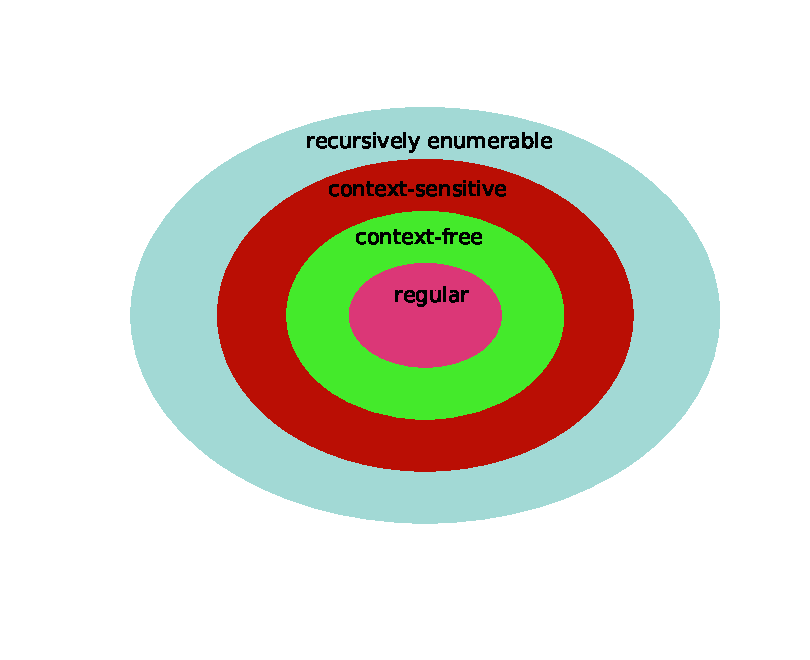
\includegraphics[width=\linewidth,keepaspectratio=true]{./figs/chomsky_h-eps}
		\fi
		\caption{\small Chomsky Hierarchy}
		\label{mtv:ch}
	\end{minipage}
\end{figure}

\subsection{Chomsky Hierarchy}\label{flt:ch}
\cite{Chomsky1956} introduced a nested hierarchy for different formal grammars of the form $C_1 \subsetneq C_2 \subsetneq C_3 \subsetneq C_4$ as shown in figure \ref{mtv:ch}. The different classes of grammar are progressively strict subsets of the class just above them in the hierarchy. These classes are not just distinguished by their rules or the languages they generate but also on the computational construct needed to decide them. We now take a closer look at the classes in this hierarchy. Please note that for each of these classes the grammar definition is G = $\langle \Sigma, NT, S, R \rangle$.
\subparagraph{Recursively Enumerable.} Any grammar decidable by an unrestricted Turning machine with no constraints on the production rules $a \rightarrow b$. (Compare to halting problem.)
\subparagraph{Context-Sensitive.} (Don't understand too well yet.)
\subparagraph{Context-Free.} Such a grammar is described by production rules of the form $A \rightarrow \alpha$ where $A \in NT$ and $\alpha \in (\Sigma \cup NT)$. Context free grammar lead to context free languages (CFL) which are hierarchical in structure, albeit it is possible that same CFL can be described by different context free grammars, leading to different hierarchical syntactic structures of the language. A CFG is decidable in cubic time of length of string by push down FSA. A psuh down automaton employs a running stack of symbols to decide its next transition. The stack can also be manipulated as a side effect of the state transition.
\subparagraph{Regular.} Characterized by production rules of the form $A \rightarrow \alpha ; A \rightarrow \alpha B$ where $\alpha \in \Sigma$ and $(A, B) \in NT$. . The non terminal in production can therefore be viewed as the next state(s) of a finite state automaton (FSA) while the terminals are the emissions. Regular grammars are decidable in linear time of length of string by a FSA.


\subsection{Subregular Hierarchy}\label{flt:sh}
The simplest class of languages encountered in section \ref{flt:ch} were regular languages that can be described using a FSA. If a language can be described by a mechanism even simpler than the FSA then it is a subregular language. While far from the expressive capabilities of regular languages which in turn are the least expressive class in the Chomsky hierarchy, subregular languages provide an excellent benchmark to test basic concept learning and pattern recognition ability of any intelligent system.

\subparagraph{Strictly local languages.} We start with a string $w$ and we are given a lookup table of k-adjacent characters known as \textit{k-factors}, drawn from a particular language. The lookup table therefore serves the role of the language description. A language is \textit{k}-local, if every \textit{k}-factor seen by a \textit{scanner} with a windows of size $k$ sliding over the string $w$, is included in the aforementioned lookup-table.  

\subparagraph{Locally k-testable languages.} Instead of sliding a scanner over \textit{k}-factors we consider all the \textit{k}-factors to be atomic and build \textit{k}-expression out of them using \textit{propositional logic}. This language description is locally k-testable. As in the case of strictly local languages, scanner won window size $K$ slides over the string and records for every k-factor in vocabulary it's occurrence or nonoccurence in the string. The output of this scanner is then fed to a boolean network which verifies the k-expressions.



